\section{判断语句}\label{sec:判断语句}
\sectionAuthor{Jiaqi Z.}

\begin{Abstract}
    \item 如何在脚本中使用\code{if}及相关语句
    \item 如何对数值、字符串和文件进行判断
    \item 如何进行逻辑判断(与、或、非)
\end{Abstract}

在之前的脚本中,我们只能按照顺序进行执行,从某种程度上来看,这并不“智能”。通常来说,一个好的脚本应该会根据实际情况来决定执行的内容,比如,当用户输入了一个文件名后,如果这个文件并不存在,程序应当做出相应的反馈。这一节,我们就会稍微了解以下如何进行判断,并且让程序根据情况做事。

\subsection{\keyword{if}语句}\label{subsec:判断语句-if语句}

在开始这一切的学习之前,让我们先来了解一个最基本的判断语句框架,以便在后面更好地讨论深入的话题。类似于C语言和Python语言等,在Shell脚本中,最简单的判断语句(\code{if}语句)框架如下:

\begin{lstlisting}[language=bash]
commands1
if [ condition ]; then
    commands2
fi
commands3
\end{lstlisting}

\begin{figure}
    \centering
    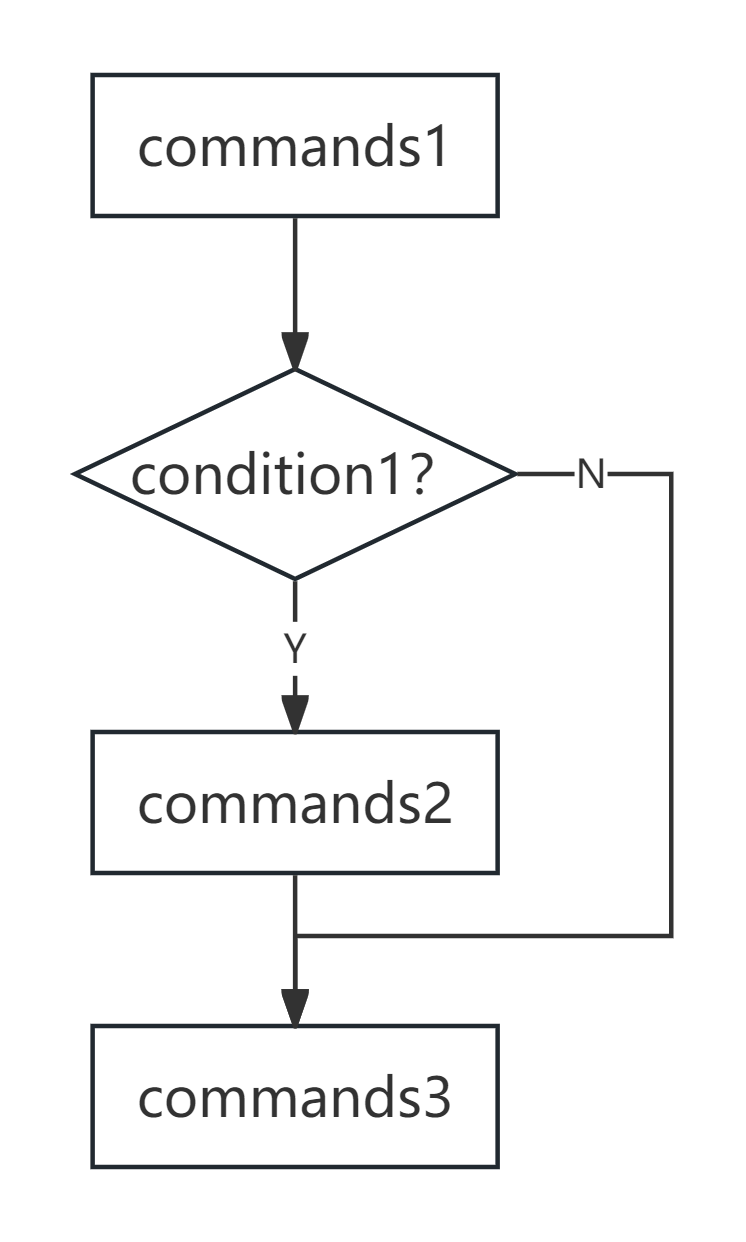
\includegraphics[width=1\linewidth]{Linux基础/Shell脚本基础/判断语句/fig/if语句.png}
    \caption{if语句流程图}
    \label{fig:判断语句-if语句流程图}
\end{figure}

这一段代码当执行完\code{commands1}之后,进行condition判断(条件是否成立),如果(if)成立,然后(then)执行\code{commands2}语句,\emph{否则不执行任何语句},最后执行\code{commands3}。

\begin{attention}
    无论条件是否满足,\code{commands3}都会执行(它是if语句之外的内容,类似于\code{commands1})。在这里的\code{commands1,commands2,commands3}都代表语句(们),每一部分可以是一条或多条语句。\code{condition}是\emph{判断条件},在后面的部分我们将详细介绍如何描述这一部分,简单来说,它描述的内容就是“是否……?”。

    需要特别注意\code{condition}前后与中括号之间的空格,这个空格不能省略!千万不要写成\code{[condition]}这种形式。
\end{attention}

\begin{extend}
    与C语言使用大括号,Python语言使用缩进不同,Shell脚本采用类似于Basic语言和MATLAB那样使用语句表示一整个语句块的方式。一个判断语句一定是以\code{if}开始,以\keyword{fi}结束。这个\code{fi}不代表“finish”或者“final if”等类似含义,而是\code{if}的倒序(在后面其他内容的学习中,会逐渐印证这一点)。

    换言之,在上述代码中,使用缩进与否并不会影响脚本执行效果,但为了增强可读性,我们仍然建议\emph{使用缩进表示每一级之间的层级关系}。事实上,如果你使用\code{vi}创建\code{*.sh}文件时,在输入\code{if}后默认会进行缩进,这也是大多数现代程序语言文本编辑器应当具有的功能。
\end{extend}

\subsection{关系运算符}\label{subsec:判断语句-关系运算符}

任何一个分支判断语句,都应当首先给定一个关系运算,并根据这个结果来判断应该执行哪些命令。在Shell脚本中,我们大致可以将关系运算符分成三类:

\subsubsection{整数比较}

类似于数学上的大于、小于和等于,在Linux当中也有对数值的比较,包括等于(\code{-eq}, \code{==})、不等于(\code{-ne}, \code{!=})、大于(\code{-gt}, \code{>})、小于(\code{-lt}, \code{<})、大于等于(\code{-ge})和小于等于(\code{-le})六种。

\begin{attention}
    在Shell脚本中,许多运算符都是通过上面这种“选项”的形式给出。与一般输入命令类似,选项前后也需要有空格进行分割。

    除了选项格式外,前四种(等于、不等于、大于和小于)我们也给出了类似于C和Python等其他编程语言所使用的运算符格式。这些在Shell脚本中同样可用。但是,对于大于等于和小于等于,没有\code{>=}和\code{<=}。如果你使用了这两个符号,大概率会报错。关于这一问题,目前还没有找到相关的解决方法,如果你有了对应解决方法(当然,不是后面要讲的内容),请联系我。
\end{attention}

\begin{extend}
    这些选项实际上是英文单词的缩写,例如,\code{eq}=equal; \code{ne}=not equal; \code{gt}=greater than; \code{lt}=less than; \code{ge}=Greater or Equal; \code{le}=Less or equal

    在后面你还会见到其他类似的语句,了解它们的实际含义可以帮助你记忆这些选项。
\end{extend}

下面的程序可以用来判断两个数字是否相等(使用前面的\code{if}语句)

\begin{lstlisting}[language=bash,caption=if\_equal,numbers=left]
#!/bin/bash
# 判断两个数字是否相等
a=10
b=10
# if语句判断是否相等
if [ $a -eq $b ]; then
    echo "$a is equal to $b"
fi
# 判断结束后输出
echo "Bye!"
\end{lstlisting}

你可以试着修改变量的值,查看输出结果是否有不同。在上述代码中,当变量相等时,判断结果为“1”,从而执行里面的语句;如果不相等,则判断结果为“0”,跳过里面的语句。无论结果如何,你都会看见第10行所输出的“Bye!”(它在\code{if}语句外面)。

\begin{extend}
    在这里我们提到了“1”和“0”,它们实际上叫做“\emph{布尔值}”或者“\emph{逻辑值}”,也是关系运算(与后面要提到的逻辑运算)的返回结果,其值只包含两种:“真”(也可以用“True”、“1”等代替)和“假”(也可以用“False”、“0”等代替)。
\end{extend}

\begin{attention}
    在中括号里面表示条件判断时,请务必记得中括号内前后要加空格,同时\code{-eq}前后也要加空格。

    在完成\code{if}语句后,不要忘记后面的\code{fi}。
\end{attention}

你也可以试着修改判断条件,例如改成\code{-gt},并修改变量的值,查看结果。

\subsubsection{*浮点数比较}

\begin{extend}
    由于前面所介绍的浮点数在脚本中的局限性,这一部分内容关于浮点数的比较并非必须了解。但如果你确实有此方面需求,在确定不能使用其他如C和Python等编程语言实现的前提下,可以参考这一部分所介绍的方法。

    相比于前面的整数比较,浮点数比较\emph{不能使用}前面的“选项”格式。例如,你写出\code{if [ 3.5 -ne 2.5 ]}是错误的。但是,前面所使用的运算符形式如\code{==, !=}等还是可用的。基于此,对于判断等于和不等于(包括大于和小于),最简单的方法就是使用如\code{if [ 3.5 != 2.5 ]}的格式。

    但是,对于大于等于和小于等于这两种情况,整数部分尚且还有选项可用,浮点数则完全没有对应的简单方法。参考前面\ref{subsec:变量-变量简单运算}一节所介绍的\code{bc}命令,我们可以退而求其次,借助于逻辑运算符的输出结果1和0,来进行判断。例如,我们希望判断3.5是否大于等于2.5,则可以使用\code{if [ \$(echo "3.5 >= 2.5" | bc) -eq 1 ]}这种方式,其中小括号部分借助管道运算符和\code{bc}命令计算\code{3.5 >= 2.5}的结果,根据前面所介绍的逻辑值,输出结果应当是0或1(在这里为1)。然后利用整数的判断方法,判断它与0或1的关系,从而实现浮点数对大于等于和小于等于的判断。
\end{extend}

\subsubsection{字符串判断}

与数值判断类似,字符串也可以进行相应的判断,一般常见的包括判断两个字符串是否相等(\code{==}),是否不相等(\code{!=}),以及判断一个字符串是否为空字符串(\code{-z}和\code{-n})

\begin{attention}
    在判断是否为空字符串时,可以使用\code{-z}和\code{-n},二者在本质上判断的内容是一样的,但返回结果\emph{相反},前者当内容为空时返回“真”,后者当内容不为空时返回“真”。借助于后面的“求非”运算,这二者只需要有一个即可,但为了简洁易读,还是建议在对应的时候使用正确的关系运算符。

    此外,与前面数值判断不同,判断字符串是否为空是“一元运算符”,即\emph{只需要一个变量}。后面的代码则给出了这种一元运算符的一般格式。
\end{attention}

下面的代码实现了判断一个字符串是否为空字符串:

\begin{lstlisting}[language=bash,caption=string\_empty,numbers=left]
#!/bin/bash
# 判断字符串是否为空
read -p "Please input a string:" string
# -n当字符串不为空时为真
if [ -n "$string" ]; then
    echo "Right! I got something ..."
    echo "You input: $string"
fi
echo "Bye!"
\end{lstlisting}

上述代码第5行通过\code{-n}判断输入字符串是否不为空,如果有内容(结果为真),则执行\code{if}语句里面的内容。

\begin{attention}
    在对字符串进行判断时(包括使用二元关系运算符),请务必将字符串变量前后加上双引号。如果不加双引号可能会造成奇怪的错误。
\end{attention}

\subsubsection{文件判断}

Shell脚本也提供了大量的运算符选项,用来判断文件的相关信息。例如,使用\code{-e}判断文件\emph{是否存在},使用\code{-f}(\code{-d})判断是否为普通文件(目录),使用\code{-r, -w, -x}依次判断文件是否可读、可写、可执行。

与前面字符串的代码类似,这里的所有运算符都是一元运算符(即采用\code{<选项> 变量}的格式。例如,下面的代码简单实现了判断文件\code{INCAR}是否存在的功能:

\begin{lstlisting}[language=bash,caption=file\_exist,numbers=left]
#!/bin/bash
# 判断文件INCAR是否存在
if [ -e "INCAR" ]; then
    echo "This file exists."
fi
echo "Bye!"
\end{lstlisting}

其中,\code{-e}后面的\code{"INCAR"}是指当前运行目录下的INCAR文件,你也可以使用绝对路径来描述文件。

\subsection{带有\keyword{else}的判断语句}\label{subsec:判断语句-带有else的判断语句}

下面,我们将进一步介绍\code{if}语句,在之前我们仅仅用来判断某一个条件是否满足,且当满足时执行某一(些)语句。但有时,我们可能有更复杂的需求。例如,判断某一个文件是否存在,如果存在则对文件进行处理,如果不存在则输出文件不存在,并提示用户重新输入。我们姑且忽略到继续输入这一动作(需要用到后面的循环),当条件不满足时如何执行另外的语句?类似于其他编程语言,在Shell当中也可以使用\code{if-else}语句。其基本格式如下:

\begin{lstlisting}[language=bash]
commands1
if [ condition ]; then
    commands2
else
    commands3
fi
commands4
\end{lstlisting}

\begin{figure}
    \centering
    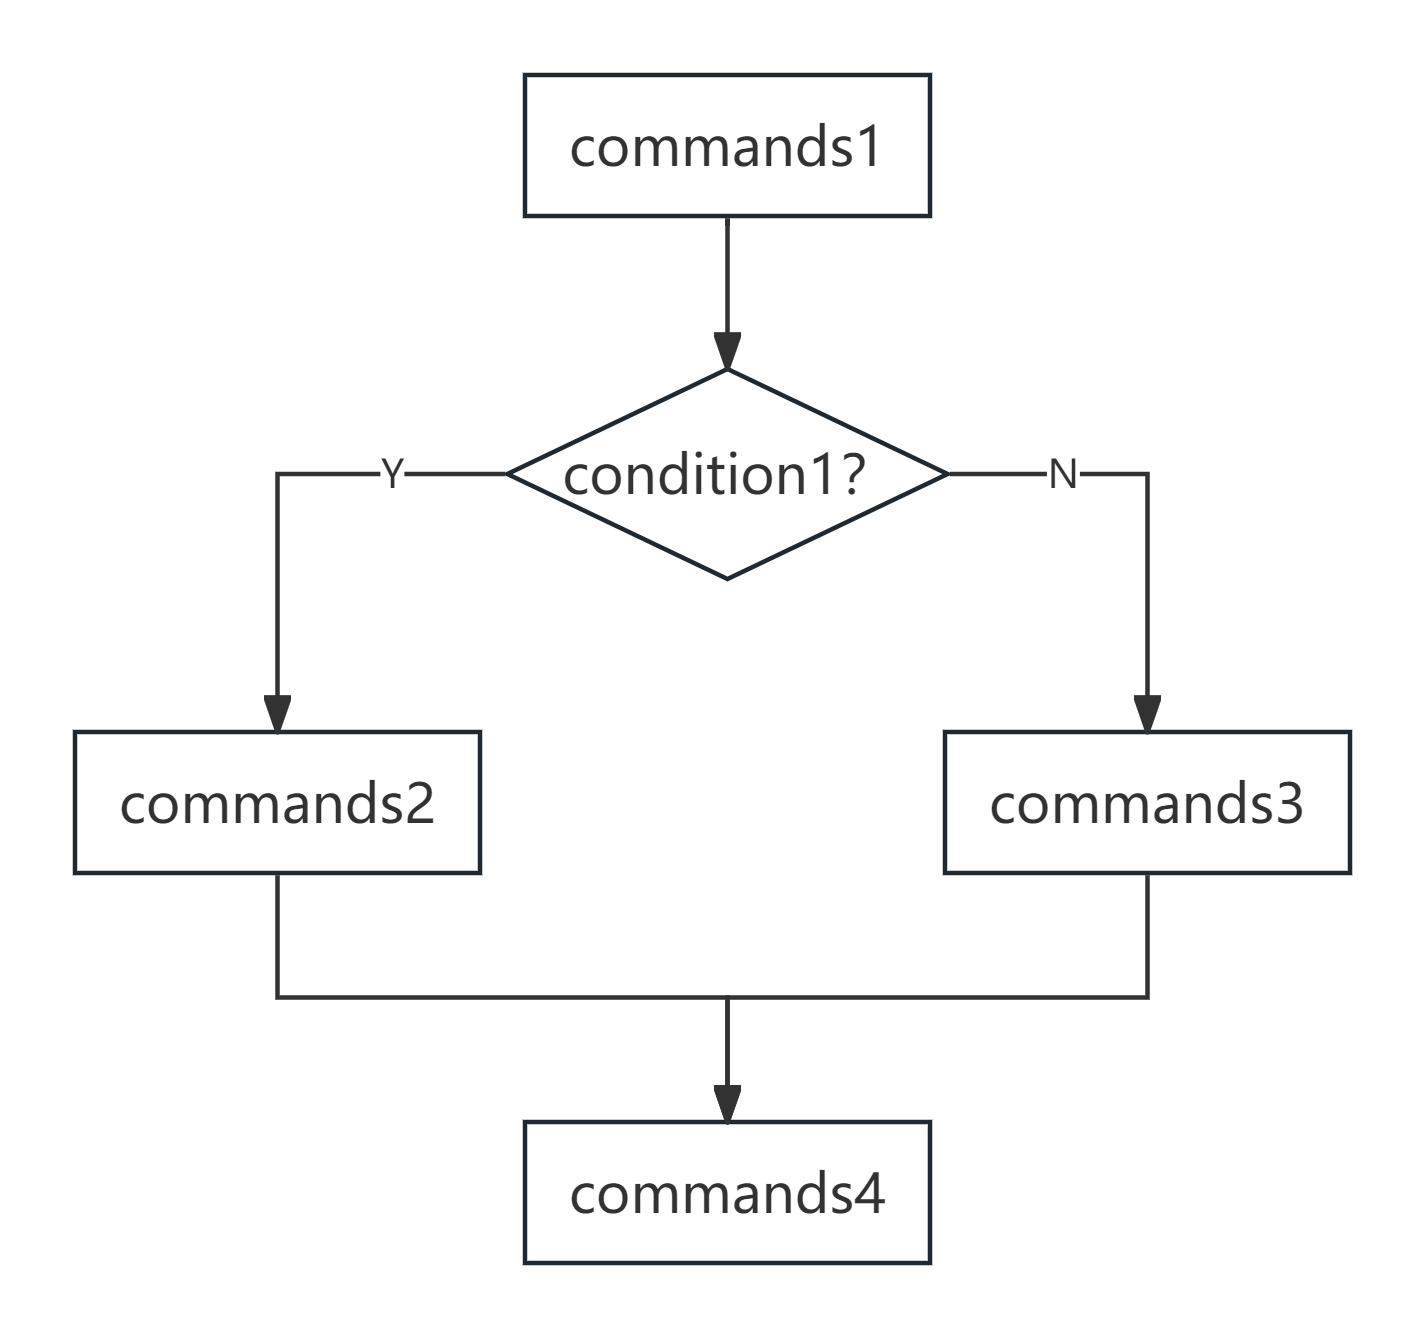
\includegraphics[width=1\linewidth]{Linux基础/Shell脚本基础/判断语句/fig/if-else语句.png}
    \caption{if-else语句}
    \label{fig:判断语句-if-else语句}
\end{figure}

首先程序会执行\code{commands1},然后进行判断,如果(if)条件成立,则(then)执行\code{commands2},否则(else)执行\code{commands3}。 无论结果如何,最后执行\code{commands4}。

下面的代码则是利用上面的语法结构,对前面的判断文件是否存在的脚本(file\_exist)进行了修改:

\begin{lstlisting}[language=bash,caption=file\_exist(2),numbers=left]
#!/bin/bash
# 判断文件INCAR是否存在
if [ -e "INCAR" ]; then
    echo "This file exists."
else
    echo "This file NOT exists."
fi
echo "Bye!"
\end{lstlisting}

除此之外,与Python语言类似,Shell脚本也有\code{if-elif-else}语句,用来对多条件进行判断,语法如下:

\begin{lstlisting}[language=bash]
commands1
if [ condition1 ]; then
    commands2
elif [ condition2 ]; then
    commands3
elif [ condition3 ]; then
    commands4
……
else
    commands5
fi
commands6
\end{lstlisting}

\begin{figure}
    \centering
    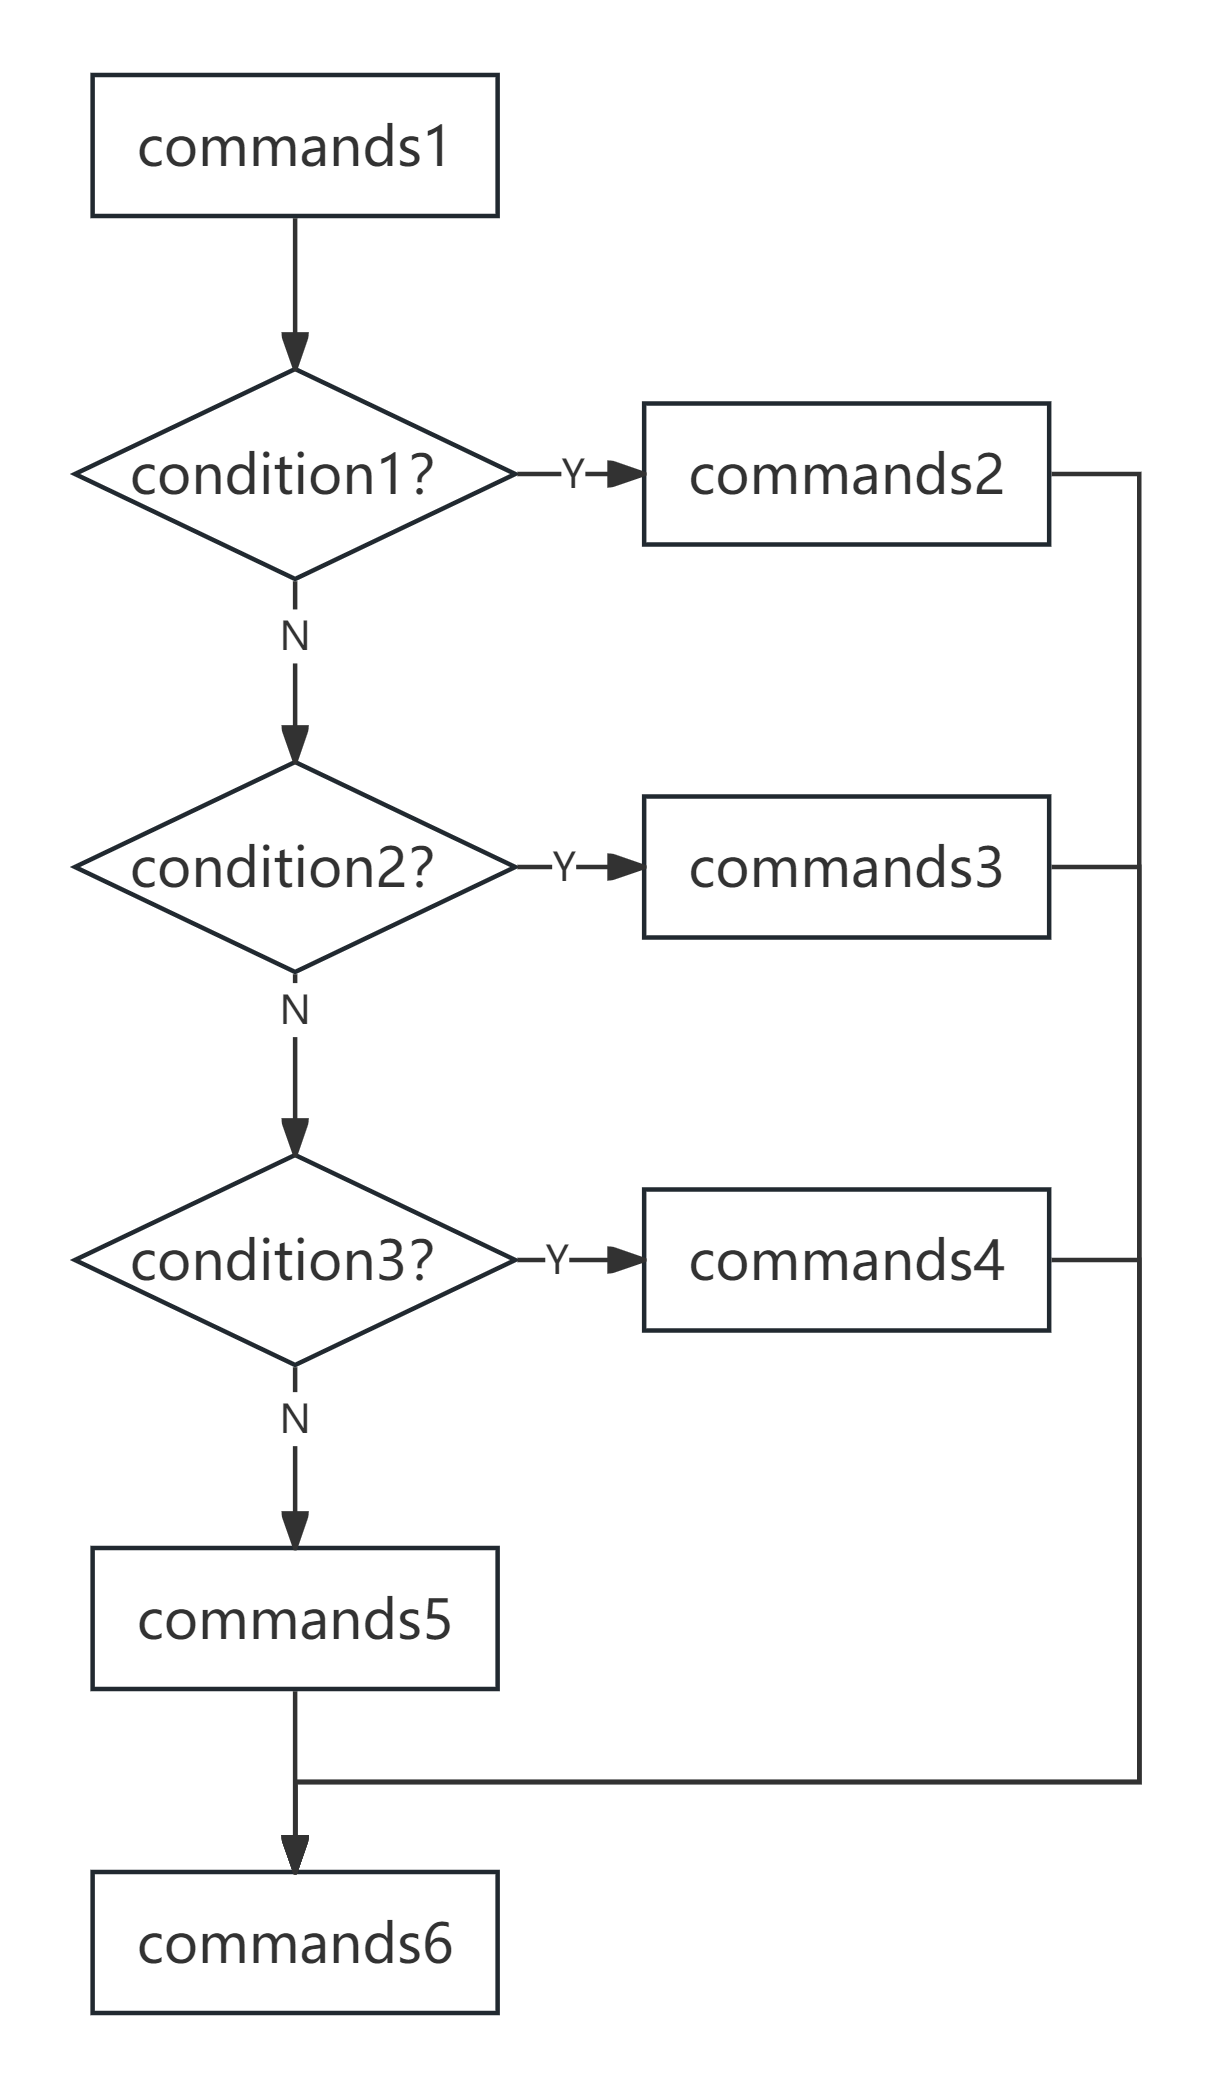
\includegraphics[width=1\linewidth]{Linux基础/Shell脚本基础/判断语句/fig/if-elif-else语句.png}
    \caption{if-elif-else语句}
    \label{fig:if-elif-else语句}
\end{figure}

程序首先判断\code{condition1}是否满足,如果(if)满足,则(then)执行\code{commands2}并结束判断语句,反之如果(else if, elif)满足\code{condition2},则(then)执行\code{commands3}并结束判断语句;反之如果……;否则都不满足(else),执行\code{commands5}。在结束判断语句后,执行\code{commands6}。

下面的程序可以用来判断两个整数之间的关系:

\begin{lstlisting}[language=bash,caption=compare\_number,numbers=left]
#!/bin/bash
# 判断两个整数之间的关系
# 输入两个整数
read -p "Please input an integer(a): " a
read -p "Please input an integer(b): " b
# 判断两个整数之间的关系
if [ $a -eq $b ]; then
    echo "$a = $b"
elif [ $a -gt $b ]; then
    echo "$a > $b"
else
    echo "$a < $b"
fi
echo "Bye!"
\end{lstlisting}

\subsection{嵌套\code{if}语句}\label{subsec:判断语句-嵌套if语句}

与其他编程语言类似,脚本也可以使用嵌套的\code{if}语句,甚至可以更复杂的\code{if-elif-else}嵌套,基于此可以实现复杂的功能。在这里我们不举例子,但有一个需要特别注意的地方:

\begin{attention}
    任何一个\code{if}语句,其后面都需要配合一个\code{fi}作为语句结束。尤其是对于嵌套时的\code{if-else}匹配问题,\code{else}总是与最近的未完成的\code{if}语句匹配(与缩进无关)。例如,下面的代码就违反了第一个原则(\code{if}必须配合有一个\code{fi});同时,看似\code{else}是属于\code{condition1}所对应的判断,但事实上是属于里面的\code{if}。

    \begin{lstlisting}
if [ condition1 ]; then
    commands1
    if [ condition2 ]; then
        commands2
else
    commands3
fi
    \end{lstlisting}

    这段代码是无法正常运行的。所缺少的\code{fi}可以加在\code{commands2}后面,也可以加在\code{commands3}后面,二者所实现的效果是不一样的。你可以尝试一下不同位置所对应的程序运行结果。

\end{attention}

\subsection{逻辑运算}\label{subsec:判断语句-逻辑运算}

在这一节的最后,让我们再来讨论一下逻辑运算。逻辑运算一共分为三种:与(\code{-a})、或(\code{-o})和非(\code{-n})。其中与运算和或运算都是二元运算符,而非运算是一元运算符。

对于与运算而言,\emph{只有当两个值都为真时结果为真}。而对于或运算,\emph{只要有一个为真,结果为真}\footnote{或者还有一种表述是,只有当两个值都为假时,结果为假。}。对于非运算,是一元运算符,其运算结果就是\emph{真变假,假变真}。

下面一个例子实现了判断三个数字是否从小大大排序:

\begin{lstlisting}[language=bash,caption=sort,numbers=left]
#!/bin/bash
# 判断三个数字是否从小到大排序
a=5
b=8
c=10
# 使用与运算符连接
if [ $a -le $b -a $b -le $c ]; then
	echo "$a, $b, $c"
fi
\end{lstlisting}

\begin{extend}
    在这里我们使用多个运算符进行连接,与其他编程语言类似,这里也具有“优先级”的问题。可以简单的理解:关系运算符的优先级高于逻辑运算符的优先级(这在大多数编程语言中都是如此)。虽然上面的写法比较简单,但对于条件复杂的时候可能不具有较好的可读性。因此,可以使用类似于C语言的运算符(\code{\&\&}表示“与”,\code{||}表示“或”),而中间每一个条件使用中括号分割,写作\code{if [ \$a -le \$b ] \&\& [ \$b -le \$c ]}
\end{extend}


\subsection{错误处理}\label{subsec:节标题-错误处理}
% 请在本节列出可能遇见的错误与解决方法

这一部分有可能出现的错误太多了,以至于难以在这里全部列出。这里仅列举一些常见的错误,且这些错误的解决方法仅是一部分可能的原因。当你出现错误时,请首先查看对应的格式是否正确,并且可以尝试联系我们。

\subsubsection{-bash: <文件名>: line <行号>: syntax error: unexpected end of file}

这是因为在使用\code{if}后没有对应的\code{fi}作为结束。通常出现在嵌套语句中或者一个\code{if}语句太长,到最后忘记了匹配。对此,我们建议,在开始就按照\code{if-fi}对应关系输入。

\subsubsection{bash: [<变量>: command not found...}

这可能是由于你在输入关系表达式时忘记了中括号里前后要加空格。

\subsubsection{-bash: [: missing `]'}
与前面的错误类似,这个通常指右中括号前面没有空格。